% !TEX root = main.tex
\section{Auswertung}
Im Folgenden werden die Auswertung der gewonnenen Daten und die Interpretation und Analyse der Ergebnisse dargelegt.
    \subsection{Beobachtung der Sonne}
    Dabei wird mit der Betrachtung der Sonne begonnen.
    Intention dessen war einerseits, die ,,antenna response function`` mittels Intensitätsmessungen zu ermitteln und
    daraus charakteristische Größen des Teleskops zu berechnen, und andererseits, als Grundlage hierfür die Annahme zu legitimieren,
    dass die Sonne innerhalb dieses Versuchs als Punktquelle aufgefasst wird.\\

    Um die Messungen der Intensitätsspektren der Sonne nicht durch charakteristische Radiostrahlung der
    21-\si{\centi \metre}-Linie zu beeinflussen,
    wurden die Messungen bei einer Freqeunz von $\SI{1420}{\mega \hertz}$ gemessen.
    Genauer wurde der Messprozess bereits in Abschnitt \ref{sec:Aufbau} beschrieben. 
    Aus den gewonnenen Spektren wurde anschließend stets der Intensitätswert bei $\SI{1420}{\mega \hertz}$ ausgelesen und in den entsprechenden Abbildungen \ref{fig:Sonnenabbild} bis \ref{fig:Sonnenkreuz_Alt} geplottet. 
    Zur Einheit der Intensität sei angemerkt, dass diese stets in ,,arbitrary units`` bzw. in \SI{}{\kelvin} angegeben wurden,
    da eine Kalibrierung des Teleskops für Absolutwerte vom \textsc{Onasala Space Observatory} nicht vorgenommen wurde.
    Allerdings genügt für die geforderten Belange eine Betrachtung der relativen Werte.\\

    \subsubsection{Raster-Scan der Sonne}
    Zunächst wurde ein Raster-Scan der Sonne vorgenommen, dabei wurden 25 Messungen zwischen $\SI{-10}{\degree}$ und $\SI{10}{\degree}$ azimuthalem und Höhenoffset in $\SI{5}{\degree}$-Schritten durchgeführt.
    Die entsprechenden jeweiligen Intensitätsmaxima wurden in Abbildung \ref{fig:Sonnenabbild} über den Relativwinkeln zur Sonne bei $\SI{0}{\degree}$ aufgetragen.
    \begin{figure}[H]
        \centering
        % GNUPLOT: LaTeX picture with Postscript
\begingroup
  % Encoding inside the plot.  In the header of your document, this encoding
  % should to defined, e.g., by using
  % \usepackage[cp1252,<other encodings>]{inputenc}
  \inputencoding{cp1252}%
  \makeatletter
  \providecommand\color[2][]{%
    \GenericError{(gnuplot) \space\space\space\@spaces}{%
      Package color not loaded in conjunction with
      terminal option `colourtext'%
    }{See the gnuplot documentation for explanation.%
    }{Either use 'blacktext' in gnuplot or load the package
      color.sty in LaTeX.}%
    \renewcommand\color[2][]{}%
  }%
  \providecommand\includegraphics[2][]{%
    \GenericError{(gnuplot) \space\space\space\@spaces}{%
      Package graphicx or graphics not loaded%
    }{See the gnuplot documentation for explanation.%
    }{The gnuplot epslatex terminal needs graphicx.sty or graphics.sty.}%
    \renewcommand\includegraphics[2][]{}%
  }%
  \providecommand\rotatebox[2]{#2}%
  \@ifundefined{ifGPcolor}{%
    \newif\ifGPcolor
    \GPcolorfalse
  }{}%
  \@ifundefined{ifGPblacktext}{%
    \newif\ifGPblacktext
    \GPblacktexttrue
  }{}%
  % define a \g@addto@macro without @ in the name:
  \let\gplgaddtomacro\g@addto@macro
  % define empty templates for all commands taking text:
  \gdef\gplbacktext{}%
  \gdef\gplfronttext{}%
  \makeatother
  \ifGPblacktext
    % no textcolor at all
    \def\colorrgb#1{}%
    \def\colorgray#1{}%
  \else
    % gray or color?
    \ifGPcolor
      \def\colorrgb#1{\color[rgb]{#1}}%
      \def\colorgray#1{\color[gray]{#1}}%
      \expandafter\def\csname LTw\endcsname{\color{white}}%
      \expandafter\def\csname LTb\endcsname{\color{black}}%
      \expandafter\def\csname LTa\endcsname{\color{black}}%
      \expandafter\def\csname LT0\endcsname{\color[rgb]{1,0,0}}%
      \expandafter\def\csname LT1\endcsname{\color[rgb]{0,1,0}}%
      \expandafter\def\csname LT2\endcsname{\color[rgb]{0,0,1}}%
      \expandafter\def\csname LT3\endcsname{\color[rgb]{1,0,1}}%
      \expandafter\def\csname LT4\endcsname{\color[rgb]{0,1,1}}%
      \expandafter\def\csname LT5\endcsname{\color[rgb]{1,1,0}}%
      \expandafter\def\csname LT6\endcsname{\color[rgb]{0,0,0}}%
      \expandafter\def\csname LT7\endcsname{\color[rgb]{1,0.3,0}}%
      \expandafter\def\csname LT8\endcsname{\color[rgb]{0.5,0.5,0.5}}%
    \else
      % gray
      \def\colorrgb#1{\color{black}}%
      \def\colorgray#1{\color[gray]{#1}}%
      \expandafter\def\csname LTw\endcsname{\color{white}}%
      \expandafter\def\csname LTb\endcsname{\color{black}}%
      \expandafter\def\csname LTa\endcsname{\color{black}}%
      \expandafter\def\csname LT0\endcsname{\color{black}}%
      \expandafter\def\csname LT1\endcsname{\color{black}}%
      \expandafter\def\csname LT2\endcsname{\color{black}}%
      \expandafter\def\csname LT3\endcsname{\color{black}}%
      \expandafter\def\csname LT4\endcsname{\color{black}}%
      \expandafter\def\csname LT5\endcsname{\color{black}}%
      \expandafter\def\csname LT6\endcsname{\color{black}}%
      \expandafter\def\csname LT7\endcsname{\color{black}}%
      \expandafter\def\csname LT8\endcsname{\color{black}}%
    \fi
  \fi
    \setlength{\unitlength}{0.0500bp}%
    \ifx\gptboxheight\undefined%
      \newlength{\gptboxheight}%
      \newlength{\gptboxwidth}%
      \newsavebox{\gptboxtext}%
    \fi%
    \setlength{\fboxrule}{0.5pt}%
    \setlength{\fboxsep}{1pt}%
\begin{picture}(7200.00,5040.00)%
    \gplgaddtomacro\gplbacktext{%
    }%
    \gplgaddtomacro\gplfronttext{%
      \csname LTb\endcsname%%
      \put(963,1308){\makebox(0,0){\strut{}$-10$}}%
      \put(1773,1160){\makebox(0,0){\strut{}$-5$}}%
      \put(2583,1011){\makebox(0,0){\strut{}$0$}}%
      \put(3392,863){\makebox(0,0){\strut{}$5$}}%
      \put(4201,714){\makebox(0,0){\strut{}$10$}}%
      \put(2270,651){\rotatebox{-11}{\makebox(0,0){\strut{}azimuth offset in $\degree$}}}%
      \put(4427,746){\makebox(0,0)[l]{\strut{}$-10$}}%
      \put(4895,1004){\makebox(0,0)[l]{\strut{}$-5$}}%
      \put(5362,1261){\makebox(0,0)[l]{\strut{}$0$}}%
      \put(5830,1518){\makebox(0,0)[l]{\strut{}$5$}}%
      \put(6297,1775){\makebox(0,0)[l]{\strut{}$10$}}%
      \put(5903,960){\rotatebox{29}{\makebox(0,0){\strut{}altitude offset in $\degree$}}}%
      \put(920,1482){\makebox(0,0)[r]{\strut{}$300$}}%
      \put(920,1972){\makebox(0,0)[r]{\strut{}$400$}}%
      \put(920,2462){\makebox(0,0)[r]{\strut{}$500$}}%
      \put(920,2951){\makebox(0,0)[r]{\strut{}$600$}}%
      \put(920,3441){\makebox(0,0)[r]{\strut{}$700$}}%
      \put(122,2462){\rotatebox{90}{\makebox(0,0){\strut{}temperature in $\si{}{K}$}}}%
    }%
    \gplbacktext
    \put(0,0){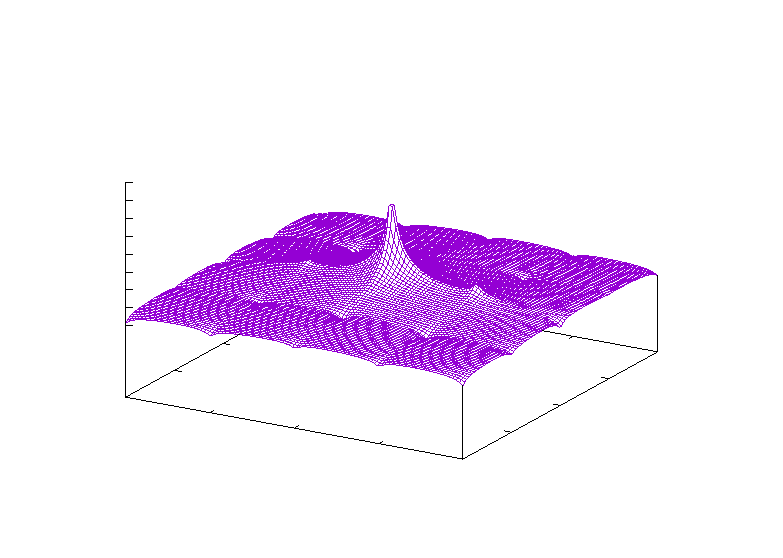
\includegraphics{plots/Sonnenabbild}}%
    \gplfronttext
  \end{picture}%
\endgroup

        \caption[Raster-Scan der Sonne]{Diese Abbildung zeigt den $5 \times 5$-Raster-Scan der Sonne. Dabei wird deutlich, dass in den dunkelblau gefärbten Bereichen von $>\vert \SI{5}{\degree}\vert$ Offset sowohl in Altitude wie in Azimuth eine Grundintensität -- hier in \si{\kelvin} gemessen -- vorliegt. Je kleiner der relative Offset zur im Zentrum fokussierten Sonne, desto höher wird der Intensitätsgradient. Die Sonne als Punktquelle aufzufassen, wird durch das ausgeprägte Intensitätsmaximum bei $\SI{0}{\degree}$ azimuthalem und Höhenoffset legitimiert. Zudem fällt auf, dass bei $\SI{0}{\degree}$ Höhenoffset und $\vert\SI{5}{\degree}\vert$ azimutalem Offset erhöhte Intensitätswerte vorliegen, was in entsprechender Altitude-Ausrichtung nicht zu erkennen ist.}
        \label{fig:Sonnenabbild}
    \end{figure}
    Die Farbskala veranschaulicht deutlich, dass in den äußeren Bereichen mit Relativwinkeln größer $\approx \vert \SI{5}{\degree}\vert$ eine Grundintensität von ca. $\SI{300}{\kelvin}$ vorliegt.
    Zum Zentrum hin nimmt die Intensität hingegen stark zu,
    wobei selbst die zentrumsnächsten Messungen bei $\vert\SI{5}{\degree}\vert$ lediglich in azimuthaler Auslenkung leichte Erhöhungen aufweisen.
    Dies lässt die oben angedeutete Annahme zu, dass die Sonne hier als Punktquelle aufgefasst werden kann.
    Auf eine Betrachtung oder Darstellung von Unsicherheiten wurde aufgrund der Übersichtlichkeit verzichtet. Zudem werden nur qualitative Aussagen getroffen, insofern sind Unsicherheitsbetrachtungen hier hinfällig.

    \subsubsection{Öffnungsfunktion des Radioteleskops}
    Zur Bestimmung der ,,antenna response function``,
    welche unter der Annahme, das Teleskop sei eine Lochblende, auch als Öffnungsfunktion verstanden werden kann,
    wurden zusätzlich jeweils in azimuthaler und altitude Koordinaten relativ zur Sonne 17 Messungen von $\SI{-16}{\degree}$ bis $\SI{16}{\degree}$ in $\SI{2}{\degree}$-Schritten durchgeführt.
    Dabei wurde die jeweils andere Koordinate auf $\SI{0}{\degree}$ fixiert.
    Die ausgelesenen Intensitätsmaxima wurden gegen den relativen Offset, bezogen auf die Sonne, aufgetragen.
    Die entsprechenden Darstellungen finden sich in Abbildung \ref{fig:Sonnenkreuz_Az} (azimuthaler Offset) und Abbildung \ref{fig:Sonnenkreuz_Alt} (altitude Offset).
    In beiden Abbildungen ist der charakteristische Verlauf der $\sinc$-Funktion zu erkennen.
    Dabei bilden sich leichte lokale Maxima im Bereich von $\vert\SI{10}{\degree}\vert$ bis $\vert\SI{15}{\degree}\vert$ (Abb. \ref{fig:Sonnenkreuz_Az}) bzw. $\vert\SI{6}{\degree}\vert$ bis $\vert\SI{10}{\degree}\vert$ (Abb. \ref{fig:Sonnenkreuz_Alt}) aus.
    \begin{figure}[H]
        \centering
        % GNUPLOT: LaTeX picture with Postscript
\begingroup
  % Encoding inside the plot.  In the header of your document, this encoding
  % should to defined, e.g., by using
  % \usepackage[cp1252,<other encodings>]{inputenc}
  \inputencoding{cp1252}%
  \makeatletter
  \providecommand\color[2][]{%
    \GenericError{(gnuplot) \space\space\space\@spaces}{%
      Package color not loaded in conjunction with
      terminal option `colourtext'%
    }{See the gnuplot documentation for explanation.%
    }{Either use 'blacktext' in gnuplot or load the package
      color.sty in LaTeX.}%
    \renewcommand\color[2][]{}%
  }%
  \providecommand\includegraphics[2][]{%
    \GenericError{(gnuplot) \space\space\space\@spaces}{%
      Package graphicx or graphics not loaded%
    }{See the gnuplot documentation for explanation.%
    }{The gnuplot epslatex terminal needs graphicx.sty or graphics.sty.}%
    \renewcommand\includegraphics[2][]{}%
  }%
  \providecommand\rotatebox[2]{#2}%
  \@ifundefined{ifGPcolor}{%
    \newif\ifGPcolor
    \GPcolorfalse
  }{}%
  \@ifundefined{ifGPblacktext}{%
    \newif\ifGPblacktext
    \GPblacktexttrue
  }{}%
  % define a \g@addto@macro without @ in the name:
  \let\gplgaddtomacro\g@addto@macro
  % define empty templates for all commands taking text:
  \gdef\gplbacktext{}%
  \gdef\gplfronttext{}%
  \makeatother
  \ifGPblacktext
    % no textcolor at all
    \def\colorrgb#1{}%
    \def\colorgray#1{}%
  \else
    % gray or color?
    \ifGPcolor
      \def\colorrgb#1{\color[rgb]{#1}}%
      \def\colorgray#1{\color[gray]{#1}}%
      \expandafter\def\csname LTw\endcsname{\color{white}}%
      \expandafter\def\csname LTb\endcsname{\color{black}}%
      \expandafter\def\csname LTa\endcsname{\color{black}}%
      \expandafter\def\csname LT0\endcsname{\color[rgb]{1,0,0}}%
      \expandafter\def\csname LT1\endcsname{\color[rgb]{0,1,0}}%
      \expandafter\def\csname LT2\endcsname{\color[rgb]{0,0,1}}%
      \expandafter\def\csname LT3\endcsname{\color[rgb]{1,0,1}}%
      \expandafter\def\csname LT4\endcsname{\color[rgb]{0,1,1}}%
      \expandafter\def\csname LT5\endcsname{\color[rgb]{1,1,0}}%
      \expandafter\def\csname LT6\endcsname{\color[rgb]{0,0,0}}%
      \expandafter\def\csname LT7\endcsname{\color[rgb]{1,0.3,0}}%
      \expandafter\def\csname LT8\endcsname{\color[rgb]{0.5,0.5,0.5}}%
    \else
      % gray
      \def\colorrgb#1{\color{black}}%
      \def\colorgray#1{\color[gray]{#1}}%
      \expandafter\def\csname LTw\endcsname{\color{white}}%
      \expandafter\def\csname LTb\endcsname{\color{black}}%
      \expandafter\def\csname LTa\endcsname{\color{black}}%
      \expandafter\def\csname LT0\endcsname{\color{black}}%
      \expandafter\def\csname LT1\endcsname{\color{black}}%
      \expandafter\def\csname LT2\endcsname{\color{black}}%
      \expandafter\def\csname LT3\endcsname{\color{black}}%
      \expandafter\def\csname LT4\endcsname{\color{black}}%
      \expandafter\def\csname LT5\endcsname{\color{black}}%
      \expandafter\def\csname LT6\endcsname{\color{black}}%
      \expandafter\def\csname LT7\endcsname{\color{black}}%
      \expandafter\def\csname LT8\endcsname{\color{black}}%
    \fi
  \fi
    \setlength{\unitlength}{0.0500bp}%
    \ifx\gptboxheight\undefined%
      \newlength{\gptboxheight}%
      \newlength{\gptboxwidth}%
      \newsavebox{\gptboxtext}%
    \fi%
    \setlength{\fboxrule}{0.5pt}%
    \setlength{\fboxsep}{1pt}%
\begin{picture}(7200.00,5040.00)%
    \gplgaddtomacro\gplbacktext{%
      \csname LTb\endcsname%%
      \put(814,704){\makebox(0,0)[r]{\strut{}$300$}}%
      \put(814,1218){\makebox(0,0)[r]{\strut{}$350$}}%
      \put(814,1733){\makebox(0,0)[r]{\strut{}$400$}}%
      \put(814,2247){\makebox(0,0)[r]{\strut{}$450$}}%
      \put(814,2762){\makebox(0,0)[r]{\strut{}$500$}}%
      \put(814,3276){\makebox(0,0)[r]{\strut{}$550$}}%
      \put(814,3790){\makebox(0,0)[r]{\strut{}$600$}}%
      \put(814,4305){\makebox(0,0)[r]{\strut{}$650$}}%
      \put(814,4819){\makebox(0,0)[r]{\strut{}$700$}}%
      \put(1434,484){\makebox(0,0){\strut{}$-15$}}%
      \put(2248,484){\makebox(0,0){\strut{}$-10$}}%
      \put(3061,484){\makebox(0,0){\strut{}$-5$}}%
      \put(3875,484){\makebox(0,0){\strut{}$0$}}%
      \put(4688,484){\makebox(0,0){\strut{}$5$}}%
      \put(5501,484){\makebox(0,0){\strut{}$10$}}%
      \put(6315,484){\makebox(0,0){\strut{}$15$}}%
      \put(4851,2813){\makebox(0,0)[l]{\strut{}FWHM $ = \SI{7.80 \pm 0.13}{\degree}$}}%
      \put(4851,3173){\makebox(0,0)[l]{\strut{}$\sigma =  \SI{3.313 \pm 0.055}{\degree}$}}%
    }%
    \gplgaddtomacro\gplfronttext{%
      \csname LTb\endcsname%%
      \put(308,2761){\rotatebox{-270}{\makebox(0,0){\strut{}Intensit\"at in willk\"urlichen Einheiten}}}%
      \put(3874,154){\makebox(0,0){\strut{}Azimutwinkelversatz relativ zur Sonne in $\si{}{\degree}$}}%
      \csname LTb\endcsname%%
      \put(5816,4646){\makebox(0,0)[r]{\strut{}Messwerte}}%
      \csname LTb\endcsname%%
      \put(5816,4426){\makebox(0,0)[r]{\strut{}\textsc{Gauss}-Fit}}%
    }%
    \gplbacktext
    \put(0,0){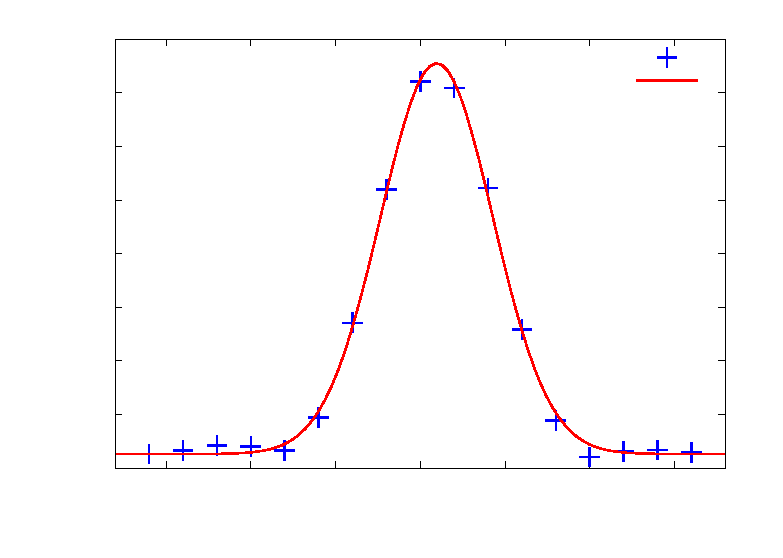
\includegraphics{plots/Sonnenkreuz_Az}}%
    \gplfronttext
  \end{picture}%
\endgroup

        \caption[Kreuz-Scan der Sonne, Azimutaler Offset]{Die Abbildung verdeutlicht den Verlauf der Datenpunkte gemäß einer $\sinc$-Funktion. Dies bestätigt die Annahme, das Radioteleskop als Lochblende aufzufassen, deren Öffnungsfunktion einer $\sinc$-Funktion entspricht. Zudem lassen sich mittels \textSC{Gauß}-Fit drei charakteristische Größen ermitteln: die Standardabweichung $\sigma$ als direktes Ergebnis des Fits mit \textsc{Gauß}scher Fehlerfunktion und die als spektrales Auflösungsvermögen zu verstehende FWHM, welche nach Formel \eqref{eq:FWHM} zu berechnen ist. Zudem kann ebenfalls direkt aus dem \textsc{Gauß}-Fit die Positioniergenauigkeit des Teleskop welche auch als intrinsische Unsicherheit $d$ verstanden wird, abgelesen werden. Sie beziffert sich auf $d = \SI{0.968 \pm 0.047}{\degree}$.}
        \label{fig:Sonnenkreuz_Az}
    \end{figure}
    \begin{figure}[H]
        \centering
        % GNUPLOT: LaTeX picture with Postscript
\begingroup
  % Encoding inside the plot.  In the header of your document, this encoding
  % should to defined, e.g., by using
  % \usepackage[cp1252,<other encodings>]{inputenc}
  \inputencoding{cp1252}%
  \makeatletter
  \providecommand\color[2][]{%
    \GenericError{(gnuplot) \space\space\space\@spaces}{%
      Package color not loaded in conjunction with
      terminal option `colourtext'%
    }{See the gnuplot documentation for explanation.%
    }{Either use 'blacktext' in gnuplot or load the package
      color.sty in LaTeX.}%
    \renewcommand\color[2][]{}%
  }%
  \providecommand\includegraphics[2][]{%
    \GenericError{(gnuplot) \space\space\space\@spaces}{%
      Package graphicx or graphics not loaded%
    }{See the gnuplot documentation for explanation.%
    }{The gnuplot epslatex terminal needs graphicx.sty or graphics.sty.}%
    \renewcommand\includegraphics[2][]{}%
  }%
  \providecommand\rotatebox[2]{#2}%
  \@ifundefined{ifGPcolor}{%
    \newif\ifGPcolor
    \GPcolorfalse
  }{}%
  \@ifundefined{ifGPblacktext}{%
    \newif\ifGPblacktext
    \GPblacktexttrue
  }{}%
  % define a \g@addto@macro without @ in the name:
  \let\gplgaddtomacro\g@addto@macro
  % define empty templates for all commands taking text:
  \gdef\gplbacktext{}%
  \gdef\gplfronttext{}%
  \makeatother
  \ifGPblacktext
    % no textcolor at all
    \def\colorrgb#1{}%
    \def\colorgray#1{}%
  \else
    % gray or color?
    \ifGPcolor
      \def\colorrgb#1{\color[rgb]{#1}}%
      \def\colorgray#1{\color[gray]{#1}}%
      \expandafter\def\csname LTw\endcsname{\color{white}}%
      \expandafter\def\csname LTb\endcsname{\color{black}}%
      \expandafter\def\csname LTa\endcsname{\color{black}}%
      \expandafter\def\csname LT0\endcsname{\color[rgb]{1,0,0}}%
      \expandafter\def\csname LT1\endcsname{\color[rgb]{0,1,0}}%
      \expandafter\def\csname LT2\endcsname{\color[rgb]{0,0,1}}%
      \expandafter\def\csname LT3\endcsname{\color[rgb]{1,0,1}}%
      \expandafter\def\csname LT4\endcsname{\color[rgb]{0,1,1}}%
      \expandafter\def\csname LT5\endcsname{\color[rgb]{1,1,0}}%
      \expandafter\def\csname LT6\endcsname{\color[rgb]{0,0,0}}%
      \expandafter\def\csname LT7\endcsname{\color[rgb]{1,0.3,0}}%
      \expandafter\def\csname LT8\endcsname{\color[rgb]{0.5,0.5,0.5}}%
    \else
      % gray
      \def\colorrgb#1{\color{black}}%
      \def\colorgray#1{\color[gray]{#1}}%
      \expandafter\def\csname LTw\endcsname{\color{white}}%
      \expandafter\def\csname LTb\endcsname{\color{black}}%
      \expandafter\def\csname LTa\endcsname{\color{black}}%
      \expandafter\def\csname LT0\endcsname{\color{black}}%
      \expandafter\def\csname LT1\endcsname{\color{black}}%
      \expandafter\def\csname LT2\endcsname{\color{black}}%
      \expandafter\def\csname LT3\endcsname{\color{black}}%
      \expandafter\def\csname LT4\endcsname{\color{black}}%
      \expandafter\def\csname LT5\endcsname{\color{black}}%
      \expandafter\def\csname LT6\endcsname{\color{black}}%
      \expandafter\def\csname LT7\endcsname{\color{black}}%
      \expandafter\def\csname LT8\endcsname{\color{black}}%
    \fi
  \fi
    \setlength{\unitlength}{0.0500bp}%
    \ifx\gptboxheight\undefined%
      \newlength{\gptboxheight}%
      \newlength{\gptboxwidth}%
      \newsavebox{\gptboxtext}%
    \fi%
    \setlength{\fboxrule}{0.5pt}%
    \setlength{\fboxsep}{1pt}%
\begin{picture}(7200.00,5040.00)%
    \gplgaddtomacro\gplbacktext{%
      \csname LTb\endcsname%%
      \put(814,704){\makebox(0,0)[r]{\strut{}$300$}}%
      \put(814,1218){\makebox(0,0)[r]{\strut{}$350$}}%
      \put(814,1733){\makebox(0,0)[r]{\strut{}$400$}}%
      \put(814,2247){\makebox(0,0)[r]{\strut{}$450$}}%
      \put(814,2762){\makebox(0,0)[r]{\strut{}$500$}}%
      \put(814,3276){\makebox(0,0)[r]{\strut{}$550$}}%
      \put(814,3790){\makebox(0,0)[r]{\strut{}$600$}}%
      \put(814,4305){\makebox(0,0)[r]{\strut{}$650$}}%
      \put(814,4819){\makebox(0,0)[r]{\strut{}$700$}}%
      \put(1434,484){\makebox(0,0){\strut{}$-15$}}%
      \put(2248,484){\makebox(0,0){\strut{}$-10$}}%
      \put(3061,484){\makebox(0,0){\strut{}$-5$}}%
      \put(3875,484){\makebox(0,0){\strut{}$0$}}%
      \put(4688,484){\makebox(0,0){\strut{}$5$}}%
      \put(5501,484){\makebox(0,0){\strut{}$10$}}%
      \put(6315,484){\makebox(0,0){\strut{}$15$}}%
      \put(4688,2864){\makebox(0,0)[l]{\strut{}FWHM $= \SI{5.63 \pm 0.12}{\degree}$}}%
      \put(4688,3276){\makebox(0,0)[l]{\strut{}$\sigma =  \SI{2.389 \pm 0.052}{\degree}$}}%
    }%
    \gplgaddtomacro\gplfronttext{%
      \csname LTb\endcsname%%
      \put(308,2761){\rotatebox{-270}{\makebox(0,0){\strut{}Kontinuums Intensität in willkürlichen Einheiten}}}%
      \put(3874,154){\makebox(0,0){\strut{}Höhenwinkelversatz relativ zur Sonne in $\si{}{\degree}$}}%
      \csname LTb\endcsname%%
      \put(5816,4646){\makebox(0,0)[r]{\strut{}Messwerte}}%
      \csname LTb\endcsname%%
      \put(5816,4426){\makebox(0,0)[r]{\strut{}\textsc{Gauss}-Fit}}%
    }%
    \gplbacktext
    \put(0,0){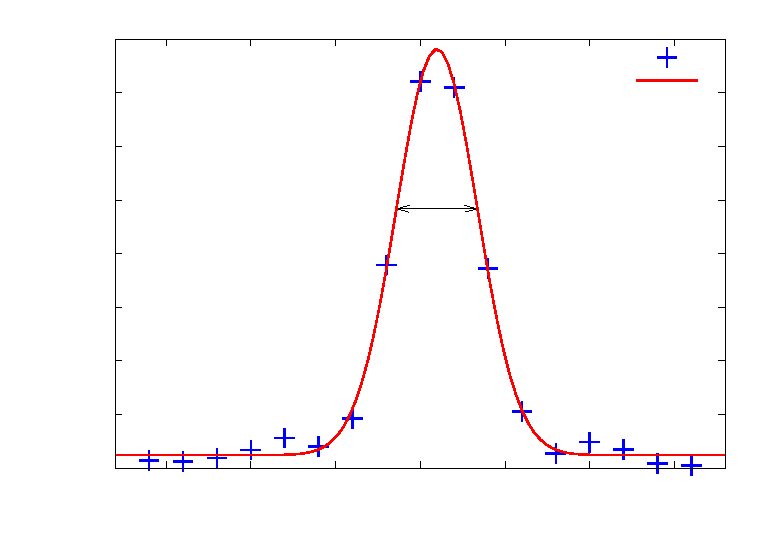
\includegraphics{plots/Sonnenkreuz_Alt}}%
    \gplfronttext
  \end{picture}%
\endgroup

        \caption[Kreuz-Scan der Sonne, Altitude Offset]{Analog zu Abbildung \ref{fig:Sonnenkreuz_Az} ist hier die Messung bei variiertem Altitude-Offset dargestellt. Die Standardabweichung, FWHM, sowie die intrinsische Unsicherheit ($d = \SI{0.984 \pm 0.048}{\degree}$) berechnen sich entsprechend.}
        \label{fig:Sonnenkreuz_Alt}
    \end{figure}
    An die Datenpunkte wurde jeweils eine \textsc{Gauß}-Funktion angefittet, welcher dann weitere Berechnungen folgten.
    % Welcher Parameter????
    Der Erwartungswert $d$ lässt einen Rückschluss auf Abweichungen in der Positioniergenauigkeit des Teleskops zu und kann hier somit als intrinsische Unsicherheit aufgefasst werden.
    Diese umfasst beispielsweise äußere Einflüsse, wie ein Zittern des Teleskops aufgrund von Wind oder auch der Umstand, dass das Teleskop in Schritten von $\SI{0.125}{\degree}$ trackt \cite{Usermanual}. Auch die Erdrotation ruft eine Winkeländerung mit $\approx \SI{0.25}{\degree}$ pro Minute hervor.
    Diese ,,tracking accuracy`` beträgt nach \cite{Usermanual} $\SI{0.5}{\degree}$. 
    Aus den beiden Messreihen ergab sich nach Bilden des gewichteten Mittelwerts und der zugehörigen internen Unsicherheit auf Grundlage der aus den mittels \textsc{GnuPlot} gewonnenen Größen und zugehörigen Unsicherheiten ein Wert von $d = \SI{0.976 \pm 0.034}{\degree}$.
    Somit liegt der hier gefundene Wert der Positioniergenauigkeit, auch im Rahmen der berechneten Unsicherheiten, höher als der aus der Literatur erwartete Wert. 
    Dennoch lässt die korrekte Größenordnung auf eine fehlerfreie Vorgehensweise schließen.
    Es lässt sich lediglich für die weiteren Beobachtungen festhalten, dass bei den hier gegebenen Bedingungen vermutlich etwas größere Unsicherheiten vorlagen aufgrund von beispielsweise kürzeren Messzeiten, starkem Wind oder anderen Einflüssen.\\ 


    Zudem wird die Betrachtung des spektralen Auflösungsvermögens zeigen, dass sowohl die berechnete wie auch die in der Literatur angegebene ,,tracking accuracy`` deutlich unterhalb derer liegen.
    Eine entsprechende Betrachtung folgt nun.
    Aus der beim \textsc{Gauß}schen Fit gewonnenen Standardabweichung $\sigma$ konnte zunächst die Halbwertsbreite (FWHM) nach \cite{wiki:FWHM}
    \begin{align}
        \text{FWHM} = \sigma \cdot 2\sqrt{2\ln(2)} \label{eq:FWHM}
    \end{align}
    berechnet werden.
    Diese kann direkt als spektrales Auflösungsvermögen verstanden werden.
    Die entsprechenden Werte sind den beiden Abbildungen \ref{fig:Sonnenkreuz_Az} und \ref{fig:Sonnenkreuz_Alt} zu entnehmen. Hierbei wurden ebenfalls der gewichtete Mittelwert gebildet und die externe Unsicherheit bestimmt.
    Somit ergab sich ein Wert von $\text{FWHM} = \SI{6.6 \pm 1.1}{\degree}$, welcher ebenfalls auf Grundlage der berechneten Unsicherheit in guter Übereinstimmung mit dem Literaturwert von $\approx \SI{6}{\degree}$ \cite{Usermanual} liegt. 
    Dieser Wert übersteigt die vorab bestimmte intrinsische Ungenauigkeit deutlich und bestätigt somit die hinreichende Genauigkeit des Teleskops für die nachfolgend dargelegten Untersuchungen.\\

    Anhand der gewonnenen Werte des Auflösungsvermögens (FWHM) aus den beiden Messreihen konnte nach dem \textsc{Rayleigh}-Kriterium mittels folgender Gleichung zudem auf den Durchmesser $D$ des Teleskops geschlossen werden \cite{Karttunen2013}:
    \begin{align}
        \Theta &= 1.22 \, \frac{\lambda}{D} \approx \ang{;;2.52} \times \frac{\lambda}{\SI{100}{\nano \metre}} \frac{\SI{1}{\centi \metre}}{D} = \SI{70}{\degree} \, \frac{\lambda}{D}\\
        \Leftrightarrow \quad D &= \SI{70}{\degree} \, \frac{\lambda}{\theta}
    \end{align}
    Anschließend wurde der gewichtete Mittelwert der beiden berechneten Werte des Teleskopdurchmessers gebildet. Da die Grundlage der durch den \textsc{Gauß}-Fit gewonnenen Größen eine nicht geringe Anzahl an einzelnen Messwerten darstellt, wurde statt der außerordentlich groß ausfallenden internen und externen Unsicherheiten ($\approx \SI{150}{\metre}$), welche auf Grundlage der kombinierten Unsicherheiten berechnet wurden, stattdessen die Standardabweichung der berechneten Teleskopdurchmesser berechnet und als sinnvoll erachtet. Somit konnte der Durchmesser des Radioteleskops ,,Brage`` aus den erhaltenen Daten berechnet werden und beziffert sich auf $D = \SI{2.23 \pm 0.37}{\metre}$. Dieser Wert liegt ebenfalls in guter Übereinstimmung zum in der Projekt-Dokumentation \cite{Usermanual} genannten Wert von $D = \SI{2.3}{\metre}$. \\    
    
    Somit kann konstatiert werden, dass die Messungen während des Versuchstags mit hinreichend großer Präzision durchgeführt und einige charakteristische Größen des Teleskops bestätigt werden konnten.